\begin{figure}
    \centering

    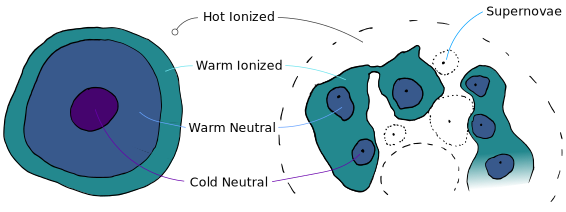
\includegraphics[width=\columnwidth]{structure.pdf}

    \caption{The three-phase structure of the ISM as proposed by \citet{Ostriker1977}.
    On the left, the small-scale structure is shown (i.e. one cloud), whereas on the right the large-scale (a top down view of a galactic disk) is shown.
    It should be noted that this figure is for illustration purposes only and does not accurately reflect the relative abundances of the phases; for a more numerical description see \citet{ferriere2001}}
    \label{fig:struct}
\end{figure}
